\section{RPC Framework} % (fold)
\label{sec:rpc_framework_structure}

The structure of the RPC framework is based around the notion of layers. 
Each layer solves a particular task, in order to achieve the goal of getting from a JavaScript stub to a C++ function, and back. Figure \ref{fig:structurediagram} shows the overall structure and interactions of each layer.

The advantages of this approach is that each layer is independent of the other. For example, if we choose a different RPC schema (i.e. something other than JSON RPC), we could easily replace the JSON RPC layer. Or, if we choose to have the C++ function on the server instead of as a Native Client module, we can easily change the transport layer to use AJAX requests or Web Sockets. 


The other advantage to this approach is that because the layers are independent and each layer has a simple interface, each layer can easily be tested. For example, to test the implementation of the run time layer, we can easily mock the JSON RPC layer, since we know its public interface.

In the end, we have four layers: the stub layer, runtime layer, JSON RPC layer and transport layer. 

\begin{itemize}
  \item Stub layer: This is responsible for parameter and result (de-)marshalling. Eventually, it calls methods in the runtime layer.
  \item Runtime layer: This manages RPC requests and responses, matching responses with requests and calling the correct callbacks.
  \item RPC Layer: This implements an RPC protocol such as JSON RPC.
  \item Transport layer: This allows messages to be sent and received between the JavaScript and C++ runtimes.
\end{itemize}

Each layer is described in detail below.

\begin{figure}
    \centering
    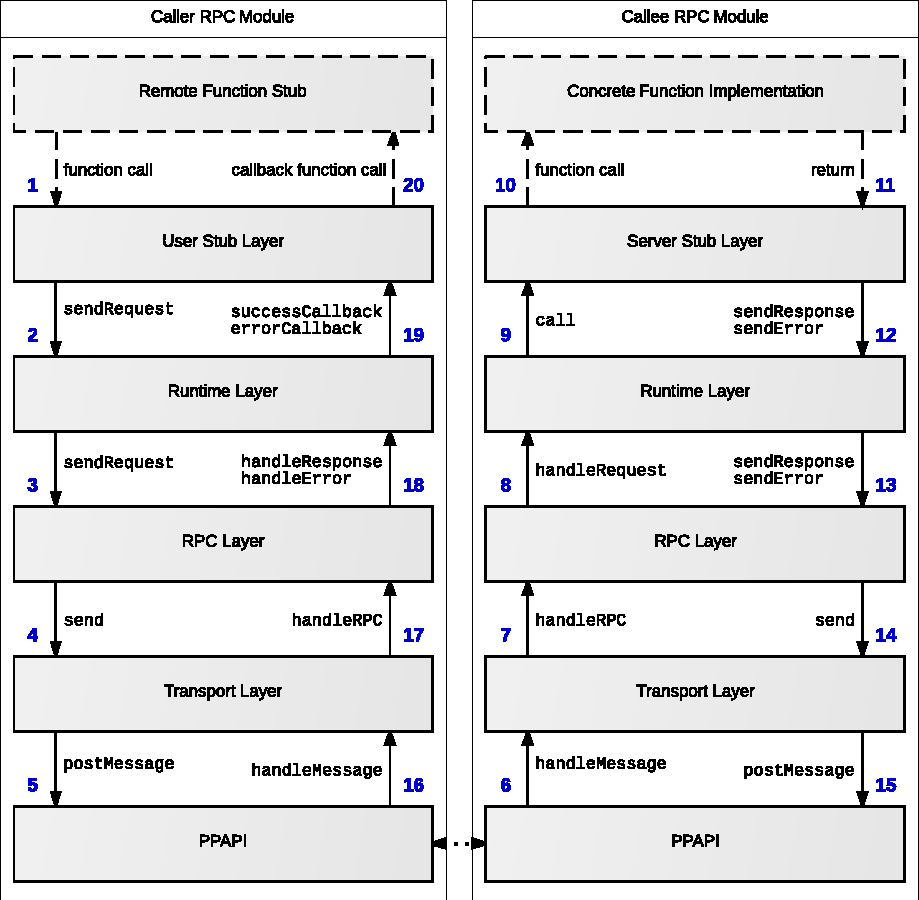
\includegraphics[width=1\textwidth]{rpc-structure-layers.pdf} 
    \caption{A layered approach to RPC. Numbering shows message flow.}
    \label{fig:structurediagram}
\end{figure}


\subsection{Transport layer} % (fold)
\label{sub:transport_layer_design}
The role of the transport layer is to implement the transportation of messages. Messages could be anything, JavaScript objects, strings, or even binary data. Moreover, the receiver could be anything - a node.js server, or a Native Client module. Finally, the transport could use any transport mechanism - web sockets, HTTP/AJAX, WebRTC, postMessage, etc.

The important thing is that the transport must provide:
\begin{itemize}
	\item An asynchronous API (should be non-blocking)
	\item The following public API:
	\begin{itemize}
		\item a \lstinline+send+ function, that accepts a payload of any type.
		\item a constructor which sets a message handler.
		\item the message handler must be invoked when a message is received. 
	\end{itemize}
\end{itemize}

The reason this approach was taken was to allow any possibility of executing remote procedure calls. It also allows the transport layer to be testable, since no concrete implementations of the layers above or below the transport layer need to be provided to test the functionality of the transport layer.


\subsubsection{Implementing the Transport Layer in JavaScript} % (fold)
\label{ssub:implementing_the_transport_layer_in_javascript}
To implement the transport layer using a Native Client module, we first encapsulate the details of a Native Client module into its own class, called \lstinline{NaClModule}. This class essentially does all the DOM manipulation for a module. To explain this, consider how a Native Client module is normally embedded in the page (as described in the background section \ref{sub:nacl_modules_ppapi} on page \pageref{sub:nacl_modules_ppapi}). The module is embedded onto the page using an \lstinline{embed} tag. The \lstinline{src} attribute points to the location of the NaCl Manifest - which tells the browser which (p)nacl executable to load. For example, \lstinline{<embed src="myModule.nmf" type="application/x-nacl" />}. The \lstinline{type} attribute tells the browser what MIME type the executable is. This could take values of either \lstinline{x-nacl} for NaCl modules or \lstinline{x-pnacl} for PNaCl modules. 

All this detail is configured through the NaClModule constructor, which takes in an object for configuration. In other words, the same \lstinline{embed} tag is created (but not actually placed on the page \emph{yet}), using the following code:

\lstset{language=JavaScript,caption={Constructing a NaClModule Object},label=code_construct_naclmodule}
\begin{code}
var myModule = new NaClModule({
  src: 'rpc-module.nmf', 
  name: 'rpc', 
  id: "MyModule", 
  type: 'application/x-pnacl'
});
\end{code}

However, much of the details of this can be `inferred' using the name of the module:

\lstset{language=JavaScript,caption={Construct a NaClModule using attribute inference},label=code_construct_naclmodule_attrinf}
\begin{code}
// creates an embed tag with the same attributes
var myModule = new NaClModule({"name": "MyModule"});
\end{code}

The attributes are inferred by using the NaClConfig global object, or a default config object if one does not exist. The id attribute is the same as the name attribute. The name and the type are inferred using the config object. Listing \ref{code_naclconfig_example} shows an example of a config object and the corresponding embed attributes.

\lstset{language=JavaScript,caption={Setting a NaClConfig object},label=code_naclconfig_example}
\begin{code}
// the NaClConfig object is a global object. 
// If required keys aren't found here, they are looked up in a 
// default config object, defined inside the framework.
window.NaClConfig = {
  TOOLCHAIN: "pnacl",
  CONFIG: "Debug"
};
var myModule = new NaClModule({"name": "MyModule"});

/* produced embed tag:
<embed name="MyModule"                   //using name in constructor
       src="./pnacl/Debug/MyModule.nmf"  //using config and name
       id="MyModule"                     //using name
       type="application/x-pnacl" />     //using config
*/
\end{code}

Once a NaClModule is constructed, it can be loaded using the \lstinline{load} method, which can take in an optional callback function as a parameter. The load method essentially inserts the \lstinline{embed} element into the page. Event handlers can be registered with the module by using the \lstinline{on} method. For example:

\lstset{language=JavaScript,caption={Registering different event handlers to a module},label=code_registering_event_handler}
\begin{code}
var myModule = new NaClModule({"name": "MyModule"});
myModule.on('load', function(){...});
myModule.on('message', function(){...});
myModule.on('crash', function(){...});
...
\end{code}

The NaClModule class therefore makes it easy to create and alter the HTML embed tag using only JavaScript. 

\begin{figure}
    \centering
    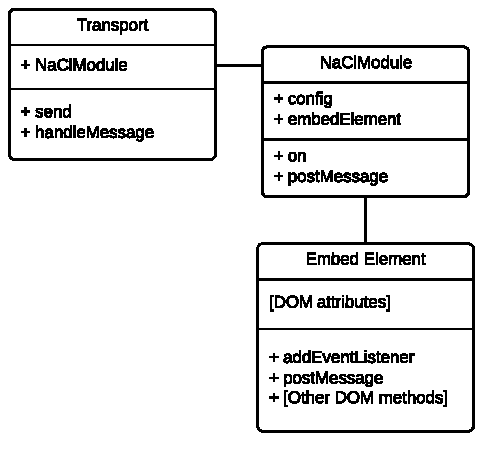
\includegraphics[width=0.5\textwidth]{transport-module-embed-clsdgrm.pdf} 
    \caption{Class diagram showing the encapsulation of NaClModule and Embed element inside a Transport object in JavaScript}
    \label{fig:naclmodule-embed}
\end{figure}

Now, the transport layer encapsulate a NaClModule object, which is used as a low-level communication object in order to send and receive messages. 


% subsubsection implementing_the_transport_layer_in_javascript (end)

\subsubsection{Implementing the Transport Layer in C++} % (fold)
\label{ssub:implementing_the_transport_layer_in_cpp_}
Since the C++ module is a singleton, the structure of the transport in C++ is a lot simpler. Essentially, the transport is a class that extends the \lstinline{pp::Instance} class provided by the PPAPI, which we use to send and receive messages using \lstinline{pp::Instance::PostMessage} and \lstinline{pp::Instance::HandleMessage}. These methods are overridden in order to link the transport with the layer above.

\begin{figure}
    \centering
    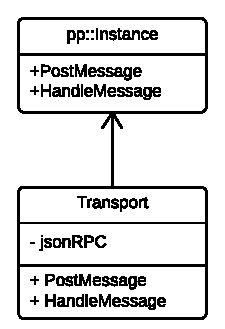
\includegraphics[width=0.25\textwidth]{transport-instance-clsdgrm.pdf} 
    \caption{Class diagram showing inheritance of \lstinline{pp::Instance} in C++}
    \label{fig:instance-transport}
\end{figure}


% subsubsection implementing_the_transport_layer_in_cpp_ (end)

% subsection transport_layer_design (end)

\subsection{RPC layer} % (fold)
\label{sub:json_rpc_layer_design}
The RPC Layer is responsible for validating messages sent and received by the transport. 

Messages \emph{received} by the transport could either be RPC \emph{requests}, \emph{responses}, or \emph{errors}. If a message is one of these three, it should forward the message to the layer above (the \emph{runtime}). An illustration of this is shown in Figure \ref{fig:rpclayer_messages_runtime}. If a message is not one of these three possibilities, the message should be ignored as it is not a RPC message.

\begin{figure}
    \centering
    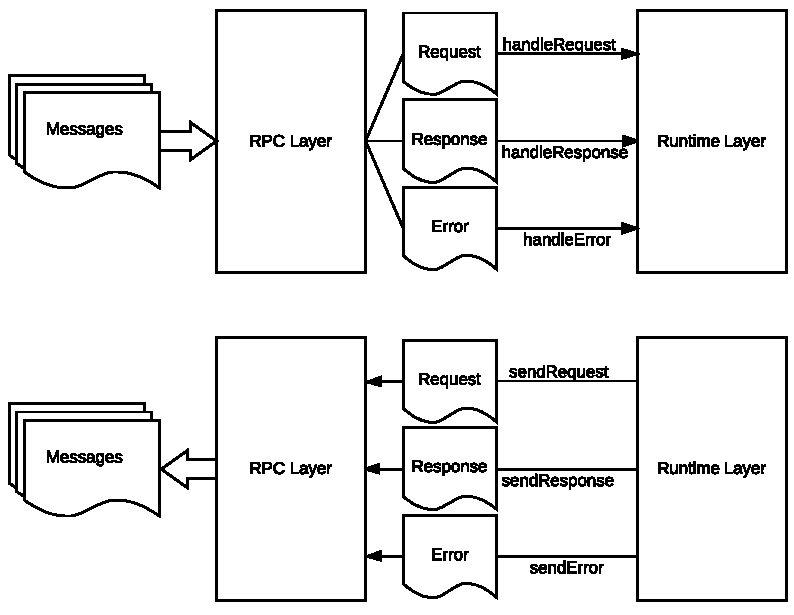
\includegraphics[width=0.8\textwidth]{rpclayer-messages-runtime.pdf} 
    \caption{Flow diagram showing how messages are filtered by the RPC layer and forwarded to the runtime layer}
    \label{fig:rpclayer_messages_runtime}
\end{figure}

The RPC layer can also provide RPC \emph{send} functions, that allow messages to be sent to the layer below. It allows RPC requests, responses and errors to be sent.

Therefore, the RPC layer has the following API:
\begin{itemize}
	\item a \lstinline+handleMessage+ function, which accepts a payload and is called by the Transport layer when a message is received. \lstinline+handleMessage+ should filter through the messages received to categorise them as requests, responses or errors. Depending on which type of message it is, the layer can call different methods of the layer above.
	\item a \lstinline+sendRequest+ function, which validates messages to be sent as requests, and forwards it down to the transport layer to be sent.
	\item a \lstinline+sendResponse+ function, which validates messages to be sent as responses, and forwards it down to the transport layer to be sent.
	\item a \lstinline+sendError+ function, which validates messages to be sent as errors, and forwards it down to the transport layer to be sent.
\end{itemize}

\subsubsection{Choosing a protocol} % (fold)
\label{ssub:choosing_a_protocol}
To implement the RPC layer, we need to choose a RPC protocol. We decided to go for the simplest protocol, which is JSON RPC. We discussed the advantages of using JSON RPC in the related work section, but there are also some benefits to do with using PPAPI to implement marshalling. Since we are using \lstinline{pp::Var}, more or less all of the JavaScript types are marshalled for us using PPAPI when we use postMessage. One alternative would have been to implement a binary based protocol, like the Ice protocol, which uses Google Protocol Buffers. There are a couple of reasons why we did not take this approach. The first is that there is an extra marshalling step in both JavaScript and C++, since we're sending and receiving binary. This adds to the complexity of both ends. The other issue is that Protocol Buffers for JavaScript aren't officially supported by Google, they are just implemented by a member of the open source community on GitHub. Finally, it is unclear whether a performance gain or loss will be achieved when we use Protocol Buffers. However, if time permitted, it would have been an interesting experiment to test different protocol implementations and measure their performance characteristics. But for now, we decided to go for the simplest approach of using JSON RPC via PPAPI.
% subsubsection choosing_a_protocol (end)

\subsubsection{Implementing the JSON RPC Layer} % (fold)
\label{ssub:implementing_the_jsonrpc_layer}
To implement the API discussed above for JSON RPC, we first need to implement validators for messages. These determine what kind of message it is - request, response, error, or none. This is done on both the JavaScript and C++ implementations, as both will have to use the protocol. Then, when a message is received, the layer simply uses these validators to check what kind of message it is. At the same time, it extracts the relevant information about the message. For example, if it is a request, it extracts the method name, parameters, etc. 

To implement the JSON RPC protocol validators, we adhere closely to the specification. Detailed unit tests are written, including passing and failing cases. The validator is then written. This is done for both the C++ and JavaScript implementations.

As well as this, some helper functions were written to create valid RPC requests, responses, and errors.

On the C++ side, a RPCRequest object is created. The RPCRequest object encapsulates generic (i.e. not necessarily JSON RPC specific) information about a RPC call. This is passed by reference to the layers that need it, so that the validation and extraction only happens once.

% subsubsection implementing_the_jsonrpc_layer (end)

% subsection json_rpc_layer_design (end)

\subsection{RPC Runtime layer} % (fold)
\label{sub:rpc_runtime_layer_design}
The main job of the runtime layer is to coordinate RPC requests and responses. As described in the background section \ref{sub:rpcruntime_background} (page \pageref{sub:rpcruntime_background}), the runtime does this by keeping track of RPC requests, and matching the requests with the responses by the use of a call identifier.

The API the runtime provides is therefore as follows:
\begin{itemize}
	\item send functions, that call the layer below.
	\begin{itemize}
		\item \lstinline+sendRequest = function(method, parameters, successCB, errorCB)+ this will give the request an ID, then keep track of that ID and the callback functions.
		\item \lstinline+sendResponse = function(id, result)+ this will just construct a response message and send it to the layer below.
		\item \lstinline+sendError = function(id, errorCode, errorMessage, errorData)+ will construct an error message and send it to the layer below.
	\end{itemize}
	\item handler functions (\lstinline+handleRequest+, \lstinline+handleResponse+, \lstinline+handleError+). The runtime will match the response's identifier with a previously sent request identifier. If a callback was provided, the callback will be called.
\end{itemize}

\subsubsection{Implementing the runtime layer} % (fold)
\label{ssub:implementing_the_runtime_layer}
The role of the runtime is different depending on the caller and the callee. Due to time constraints, the runtime has only been implemented for a JavaScript caller (client), and a C++ callee (server). However, the implementation is very similar, as it is only a language difference (in other words, the implementation in JavaScript will be the same as the implementation in C++ and vice versa).

We first consider the implementation of the caller's RPC runtime, implemented in JavaScript. To make a RPC request, the sendRequest function is called. The remote method name, parameters, success callback, and error callback are passed to this function. The runtime then constructs a RPC Request object, and gives the request a unique ID. The callbacks are added to a map of ids to callbacks. The listing below shows an example instance of a map, where two RPC requests have been made and are still waiting for responses.

\lstset{language=JavaScript,caption={An example of an  id-callback map},label=code_id_callback_map}
\begin{code}
{
  1: {
    success: function(){...},
    error: function(){...}
  },  

  2: {
    success: function(){...},
    error: function(){...}
  },  

  ...
}
\end{code}


Finally, the request object is sent. When the C++ server handles the request and sends back a response, the same ID is sent back. The JSON RPC Layer (described above) will handle the message and call one of the runtime's handlers. If it was a response, it will call the response handler. If it was an error, it will call the error handler. In either, the runtime will look for response's id inside the map. If the ID exists in the map, then the appropriate callback is called and then the key/value pair is removed from the map. The listing below shows how this is implemented for the case of a successful response.

\lstset{language=JavaScript,caption={The handle callback method in JavaScript},label=code_handle_callback_js}
\begin{code}
  RPCRuntime.prototype.handleCallback = function(rpcObject){
    // see if that id is even registered with us
    if(_.isUndefined(this.idCallbackMap[rpcObject.id])){
      logger.error("Received a callback response for invalid call");
      return false;
    }

    // get the success callback
    var successCallback = this.idCallbackMap[rpcObject.id].success;

    // call it
    if(_.isFunction(successCallback)){
      successCallback.call(null, rpcObject.result);
    }

    // delete it from the map
    this.idCallbackMap[rpcObject.id] = undefined;
    delete(this.idCallbackMap[rpcObject.id]);

    return true;
  };
\end{code}

\vspace{10 mm}

For the callee's RPC runtime, written in C++, the implementation involves finding the required function and then calling it. Since functions aren't first class citizens in C++ (unlike in JavaScript), some thought needs to be put into how to dynamically call a function. The solution we take is to define stub classes for each RPC method. The stub classes are derived from the RPCServerStub class, which has an overrideable \lstinline{virtual pp::Var call(const pp::VarArray* params, RPCError& error);} function. The \lstinline{call} function takes in the parameters and returns the result as a \lstinline{pp::Var}. In other words, all type marshalling and de-marshalling has to happen inside the \lstinline{call} function. 

When setting up the RPC Runtime object, we initialise it by adding all the functions we wish to expose. The listing below shows an example of adding RPC stubs to the runtime.

\lstset{language=C++,caption={Adding RPC stubs to the runtime},label=code_addrpcstub}
\begin{code}
// define ServerStub_MyInterface_Foo...
// ... 
// during set up...
pprpc::RPCRuntime* rpcRuntime = new pprpc::RPCRuntime(...);
rpcRuntime->AddServerStub("MyInterface::Foo", new ServerStub_MyInterface_Foo);

\end{code}

The \lstinline{AddServerStub} method works by simply maintaining a \lstinline{std::map} of \lstinline{std::string} method names to \lstinline{RPCServerStub} objects. Notice how the stubs are `flat' with respect to interfaces. What I mean here is how encapsulation is done using name mangling. This was done to simplify stubs, as in the end, interfaces are singletons which have a straightforward, static, API. In other words, since interfaces are stateless, we only represent the functions that an interface has. This greatly simplifies both the framework and code generation. However, implementing WebIDL interfaces in this way means we are limiting the implementation to only include functions (WebIDL operations), but WebIDL allows defining other interface members such as fields and constants. Since our main concern in this project was to use WebIDL to implement RPC functions we decided to stick to a simple approach of defining functions in C++, which is just through normal, namespaced function definitions in header files. The alternative, which could be a future extension, would have been to implement interfaces as classes. 

We hide the details of the ServerStub as this is discussed in the stub layer section (\ref{sub:stub_layer_design}, page \pageref{sub:stub_layer_design}).

Now that the stubs are registered with the runtime, when we receive a RPC request, the JSON RPC layer will call the runtime's \lstinline{HandleRequest} method. This will look up the string name of the function being called in the map, in order to get the corresponding RPCServerStub. If it exists, the stub's \lstinline{call} method is called.

% subsubsection implementing_the_runtime_layer (end)

% subsection rpc_runtime_layer_design (end)

\subsection{Stub Layer} % (fold)
\label{sub:stub_layer_design}
Finally, the stub layer is just a wrapper over the runtime layer's API, so that functions can be called `natively' from within the language. The stub layer also performs parameter type checking and marshalling.

\subsubsection{Implementing the stub layer} % (fold)
\label{ssub:implementing_the_stub_layer}
There is a distinction between the caller's stub layer (which we call the user stub) and the callee's stub layer (the server stub). The user stub has the job of parameter packing and calling the RPCRuntime's functions. On the other hand, the server stub is \emph{called} by the RPC runtime, and \emph{un}packs the parameter. This distinction can be seen in the RPC diagram shown in background section \ref{sec:rpc_background} on page \pageref{sec:rpc_background}.

Due to time constraints, RPC functionality has only been implemented one way, from JavaScript to C++. This means only the user stubs have been implemented on the JavaScript side, and only the server stubs have been implemented on the C++ side. We give an overview of these implementations.

The user stub implementation using JavaScript is greatly simplified due to the fact that parameter packing only involves turning a function's parameters into an array, since the server stub is expecting \lstinline{pp::Var} objects, which correspond naturally to JavaScript types. In other words, the PPAPI performs all the marshalling for us by converting JavaScript objects on the caller side into \lstinline{pp::Var} objects on the callee side.

However, to make it more useful for the JavaScript developer, the RPC framework will optionally perform \emph{type checking} on the caller side before calling the runtime. How JavaScript type checking is implemented is shown in the WebIDL bindings implementation section \ref{sub:webidl_implementation_in_javascript} on page \pageref{sub:webidl_implementation_in_javascript}, but the basic idea is the use of JSON Schemas which define the JavaScript types we are expecting.

What we want to achieve on the JavaScript side is the ability to access the defined modules, interfaces, and most importantly functions on the C++ side in the most natural way possible. We achieve this by dynamically constructing a JavaScript object that holds all this information. The object maps interface names to maps of function names to function stubs. To make this clearer, here is an example of such an object, which we shall call an RPC Module.

\lstset{language=JavaScript,caption={An example RPC Module in JavaScript},label=code_rpcmodule_example}
\begin{code}
{
  "MyInterface": {
    "foo": function(){...},
    "bar": function(){...}
  },
  "SecondInterface": {
    "fun": function(){...}
  }
}
\end{code}

Now, to call \lstinline{foo}, we call \lstinline{MyInterface.foo()}. This gives a very natural way of using RPC functions in JavaScript, as that is exactly what they are - functions! We now finally look at how the actual stub function is implemented. This happens in JavaScript stub layer's \lstinline{constructFunction} method. Essentially, it takes in a function definition as a JavaScript object, and returns a JavaScript function that is the stub. In that sense, the function definition is made \emph{declarative}, a feature which makes the generator's job (discussed later) much simpler. Here is an example of a function definition:

\lstset{language=JavaScript,caption={A function definition object},label=code_functiondef_jsstub}
\begin{code}
{
  "name": "foo",
  "params": [{"$ref": "unsigned long"}],
  "returnType": {"$ref": "boolean"}
}
\end{code}

Then, the \lstinline{constructFunction} method will take this object and use the information in it to produce a JavaScript function. The JavaScript function will do the type checking discussed earlier, but most importantly, it will call the RPC runtime to actually execute the RPC request. Here is a simplified example of a produced function:

\lstset{language=JavaScript,caption={A user stub function dynamically produced},label=code_js_stub}
\begin{code}
function(){
  // get arguments dynamically
  var args = Array.prototype.slice.call(arguments, 0);

  // the expected number of parameters is known
  // if the user gives more params, then these are probably callbacks.

  // we extract the callbacks
  var userSuccessCallback, userErrorCallback, userParams;
  if (args.length > defnParamsLength) {
    userSuccessCallback = args[defnParamsLength];
    userErrorCallback = args[defnParamsLength + 1];
  }

  // extract the user given parameters
  // now we go through each parameter and assert it is valid type

  // before calling the runtime, we alter the callback
  var callback = function (d) {
    //type checking of the result
  };


  // finally call the runtime
  return runtime.sendRequest(
    interfacePrefix+defnName, 
    userParams, 
    callback, 
    userErrorCallback
  );
}
\end{code}

To implement the C++ server stubs, we define a RPCServerStub class for each concrete function. For example, here is the \lstinline{ServerStub_MyInterface_Foo} class used in listing \ref{code_addrpcstub}.

\lstset{language=C++,caption={Defining a server stub in C++},label=code_serverstub_def}
\begin{code}
class ServerStub_StepScene : public RPCServerStub{
public:
	virtual pp::Var call(const pp::VarArray* params, RPCError& error){
		// unpack params
		// call concrete function
		// pack result, return
	}
};
\end{code}

Notice how we have combined the role of the RPC server stub to include marshalling, de-marshalling and calling the actual function implementation. This was done to simplify the framework on the C++ side, and also to expose some of the implementation details to the C++ developer. This is to allow the C++ developer to tweak the framework in order to get higher performance if they need it, or to customise a specific case. There a few cases where this might be the case. One case is when the developer wants to send and receive binary data. This is currently not supported, due to time constraints. In this case, the developer could go ahead and edit the generated code so that they can pass a \lstinline{pp::Var} to their function. Another example where this might be useful is if the developer wants to make the callback asynchronous, by creating a thread, doing computation, and sending the result at a later time. Again, this is not supported at this stage, but the developer can simply edit the \lstinline{call} function to allow this. In that sense, showing these implementation details gives power to the developer to allow them to do what they want, without forcing them to use a specific way of implementing their code.

Finally, in listing \ref{code_serverstub_def}, we purposely don't show how the parameter/result (de)marshalling happens. The implementation of this is shown in the WebIDL bindings implementation section \ref{sub:webidl_implementation_in_cpp_} on page \pageref{sub:webidl_implementation_in_cpp_}.

% subsubsection implementing_the_stub_layer (end)
% subsection stub_layer_design (end)

% section rpc_framework_structure (end)
